%\newcommand{\Exp}{\mathbb{E}}
% reset section counter
\setcounter{section}{0}

%\metadata{lecture ID}{Your names}{date}
\metadata{8}{Nicholas K. Branigan and Andrew Kirjner}{May 21, 2021}

\sec{Review and overview}

In the last lecture, we began our treatment of nonparametric density estimation with a discussion of the histogram algorithm. This intuitive approach involves constructing a histogram from our observations and normalizing it so that it constitutes a valid density function. In particular, we discuss about bias-variance trade-off:: as the bandwidth increases, the variance decreases while variance increases, and as we consider more examples, variance decreases but the bias, given its dependence on the expectation of the algorithm's predictions, does not change with the number of examples. 

In this lecture, we move to kernel density estimation, a more sophisticated technique for this problem. Then, we briefly touch parametric and nonparametric mixture models and begin our discussion of Bayesian nonparametric methods. 

\sec{Kernel density estimation}

\subsec{Introduction}
We define the kernel density estimator 
\al{
\hat{f}(x) = \frac{1}{nh} \sum_{i=1}^n K\left(\frac{x - x_i}{h}\right), \label{eq:2}
}
where $h$ is the bandwidth and $K$ is the kernel function. Recall from Lecture 1 that we have defined the kernel function to be any smooth, non-negative function $K$ such that
\als{
\int_{\R} K(x) dx = 1, \quad \int_{\R} xK(x)dx = 0, \quad \text{and} \quad \int_{\R} x^2 K(x)dx > 0.  \label{8.2}
}
Two kernel functions we have seen are the boxcar and Gaussian kernels. For the former, we now show that kernel density estimation is very similar to the histogram approach. Recall that the boxcar kernel $K(x) = \frac{1}{2} \mathbf{1}\{|x| \leq 1\}$. Thus, using the boxcar, our kernel density estimator is 
\al{
\hat{f}(x) = \frac{1}{nh} \sum_{i=1}^n \frac{1}{2} \mathbf{1}\left\{\left|\frac{x-x_i}{h}\right| \leq 1\right\}.
}
Define $B_x = \{i : |x_i - x| \leq h \}$ and let $|B_x|$ be the cardinality of this set, i.e., the number of points in $B_x$. Then we can write, 
\als{
\hat{f}(x) &= \frac{1}{nh} \sum_{i \in B_x} \frac{1}{2} \mathbf{1}\left\{\left|\frac{x-x_i}{h}\right| \leq 1\right\} \\
&= \frac{1}{nh} \sum_{i \in B_x} \frac{1}{2}\\
&= \frac{|B_x|}{2nh}. \label{eq:6}
}
To see the similarity with the histogram algorithm, recall that for the histogram,
\al{
\hat{f}(x) = \frac{\hat{p}_j}{h} = \frac{|B_j|}{nh},
}
for $x \in B_j$. Moreover, note that for the histogram, $h$ corresponds to the bin width, whereas for our boxcar density estimator, $h$ is half of the bin width. The characteristic difference between the approaches is that for kernel density estimators, our bins are not fixed but moving with and centered at $x$. 

Of course, we require that our kernel density estimator constitutes a valid density. There are two approaches for verifying that \eqref{eq:2} coheres with the definition of the probability density function. The first is to check directly that \eqref{eq:2} integrates to 1:
\al{\int_\R \hat{f}(x)dx &= \int_\R \frac{1}{nh} \sum_{i=1}^n K\left(\frac{x-x_i}{h} \right)dx \nonumber \\
&= \frac{1}{nh} \sum_{i=1}^n \int_\R K\left(\frac{x-x_i}{h} \right)dx \nonumber \\
&= \frac{1}{nh} \sum_{i=1}^n \int_\R K\left(\frac{x}{h} \right)dx \label{eq:1}\\
&= \frac{1}{nh} \sum_{i=1}^n h\int_\R K\left(z \right)dz \label{8.9}\\
&= \frac{1}{nh} \sum_{i=1}^n h \nonumber \\
&= 1. \nonumber
}
To reach \eqref{eq:1}, we used that shifting a function being integrated over the continuum by a constant has no effect on the value of the integral. In \eqref{8.9} we made a change of variables.\footnote{Let $\mathcal{R}[a, b]$ denote the set of functions that are Riemann integrable on $[a, b]$. Then, let $f \in \mathcal{R}[a, b]$ and let $g$ be a strictly increasing function from $[c, d]$ onto $[a, b]$ such that $g$ is differentiable on $[c, d]$ and $g^\prime \in \mathcal{R}[c, d]$. Then $(f \circ g) \cdot g^\prime \in \mathcal{R}[c, d]$ and $\int_a^b f(x)dx = \int_c^d f(g(t))g^\prime (t)dt$ \cite{johnsonbaugh_foundations_2010}.} 

\begin{figure}[h!]
\centering
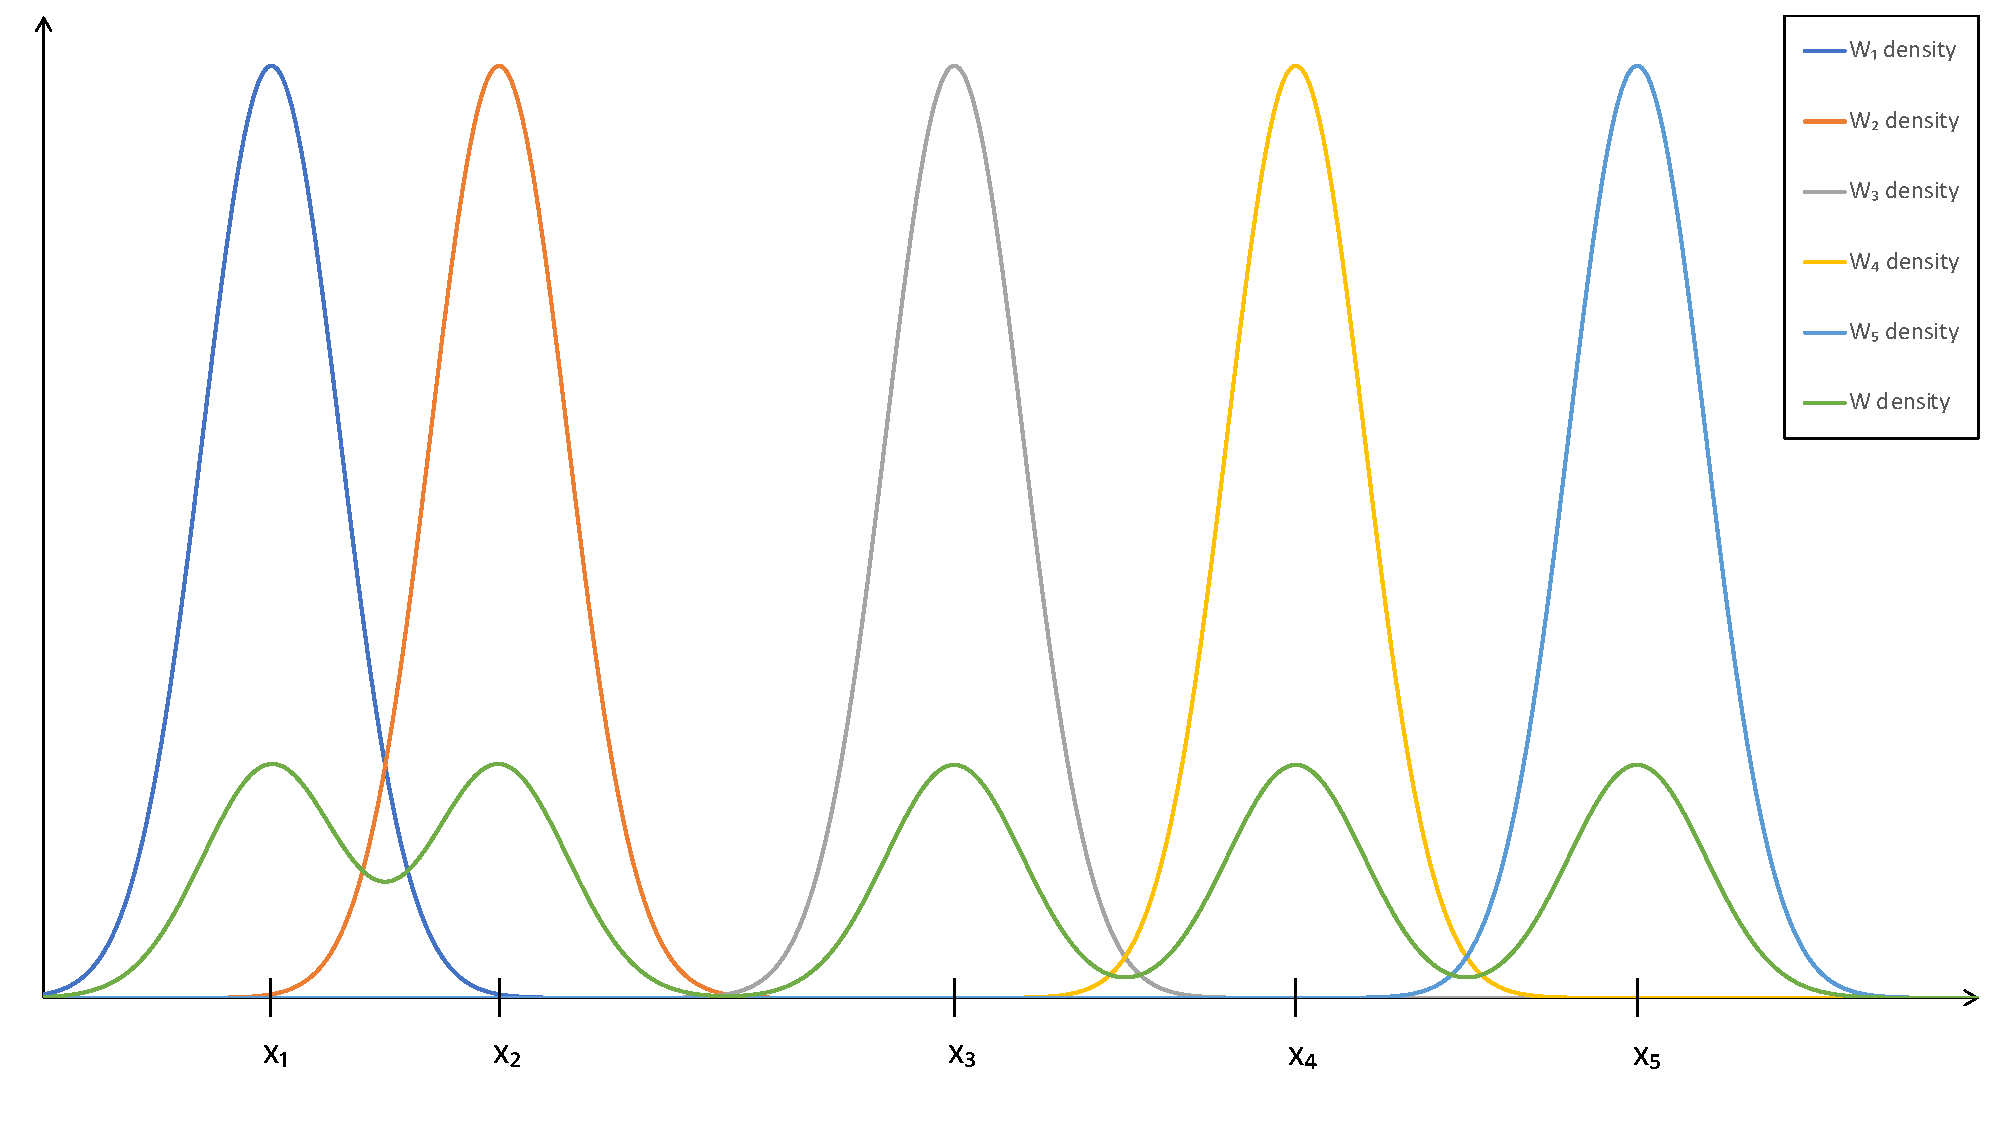
\includegraphics[width=.8\linewidth]{figure/Lecture08/fig-1.pdf}    
\caption{Example of Gaussian mixture model. In the figure above, $W = \frac{1}{5}\sum_{i=1}^5 W_i$, where $W_i \sim \cN(x_i, h^2)$. Per Theorem 8.1, the Gaussian kernel density estimator assumes that the density $\hat{f}$ is an equally weighted mixture of Gaussians centered on the observations $\{x_i\}_{i=1}^n$ with variance $h^2$.}
\end{figure}

The second approach for sanity checking our definition in \eqref{eq:2} is to view $K(x)$ as a probability density function. Examining \eqref{8.2} confirms that this is a valid move. Then, we find that $\hat{f}$ is identical to a density function as desired. The following theorem formalizes this.  

\begin{theorem}
Let $\xi \sim K(x)$, $Z \sim \mathrm{Unif}\{x_1, \dots, x_n\}$. Further, define $W = Z + \xi h$. Then, the density function of $W$ is $\hat{f}$.
\end{theorem}
\begin{proof}
Let $W_i = x_i + \xi h $ for each $i \in \{1, \dots, n\}$. Finding the density of $W_i$ is straightforward. To do this, we first find the distribution function of $W_i$:
\als{
F_{W_i}(x) &= P\{W_i \leq x\}\\
&= P\{x_i + \xi h \leq x\}\\
&= P\left\{\xi \leq \frac{x - x_i}{h}\right\}\\
&= F_\xi \left(\frac{x - x_i}{h}\right).
}
Then, we differentiate to find the density:
\als{
f_{W_i}(x) &= \frac{d}{dx} F_{W_i}(x)\\
&= \frac{d}{dx} F_\xi \left(\frac{x - x_i}{h}\right)\\
&= f_\xi \left( \frac{x - x_i}{h} \right)\frac{1}{h}\\
&= \frac{1}{h}K\left( \frac{x - x_i}{h}\right).
}
Now, since $W = W_i$ with probability $\frac{1}{n}$, we can easily find the density of $W$. We again appeal to distribution functions to show this.
\al{
F_W(x) &= P\{W \leq x\} \nonumber \\
&= \tfrac{1}{n}P\{W_1 \leq x\} + \dots + \tfrac{1}{n}P\{W_n \leq x\} \nonumber \\
&= \tfrac{1}{n}F_{W_1}(x) + \dots + \tfrac{1}{n}F_{W_n}(x). \label{eq:3}
}
Differentiating \eqref{eq:3} gives that 
\als{
f_W(x) &= \frac{1}{n}\sum_{i=1}^n f_{W_i}(x)\\
&= \frac{1}{nh}\sum_{i=1}^n K\left( \frac{x - x_i}{h}\right)\\
&= \hat{f}(x).
}
(If $W$ were not a mixture of random variables but a sum of them, computing its density would be far more complicated.)
\end{proof}

\subsec{Integrated risk}

Now, we turn to the risk associated with the Gaussian kernel density estimator.
\begin{theorem}
For the Gaussian kernel density estimator the risk is 
\al{
R\left(f, \hat{f}\right) = \underbrace{\frac{1}{4}\sigma_k^2 h^4 \int  f^{\prime \prime} (x)^2 dx}_{\text{bias}} + \underbrace{\vphantom{\int}\frac{\beta_k^2}{nh}}_{\sigma^2} + \cO \left(h^6\right) + \cO \left(n^{-1} \right), \label{eq:4}
}
where $\sigma_k^2 = \int x^2 K(x)dx$ and $\beta_k^2 = \int K(x)^2 dx$. The first term in \eqref{eq:4} is the bias and the second is the variance.
\end{theorem}
Recall that for the histogram density estimator, 
\al{
R\left(\hat{f}, f\right) &= \underbrace{\frac{h^2}{12}\int  f^\prime(x)^2 dx}_{\text{bias}} + \underbrace{\vphantom{\int}\frac{1}{nh}}_{\sigma^2} + \cO(h^2) + \cO(n^{-1}). \label{eq:5}
}
Comparing \eqref{eq:4} and \eqref{eq:5}, we see that for the Gaussian kernel density estimator, we want $f^{\prime \prime}(x)$ to be small rather than $f^{\prime}(x)$. More importantly, for values of $h < 1$, the bias of the Gaussian kernel density estimator will be lower than for the histogram estimator. We encounter the usual bias-variance tradeoff here: increasing $h$ results in more smoothing which boosts bias and depresses variance whereas decreasing $h$ results in less smoothing which depresses bias and boosts variance. 

By minimizing the risk with respect to $h$, we find the optimal bandwidth
\al{
h^* &= \left( \frac{\beta_k^2}{\sigma_k^2 A(f) n}\right)^{1/5}, \quad \text{where} \quad A(f) = \int f^{\prime \prime}(x)^2dx. \label{8.28}
}
As usual, the optimal bandwidth is inversely dependent on $n$. Plugging $h^{*}$ into \eqref{eq:4}, we find that as a function of $n$, $R(f, \hat{f}) \propto \cO(n^{-4/5})$. We observe that this is an improvement over the histogram estimator where as a function of $n$, $R(f, \hat{f}) \propto \cO(n^{-2/3})$. 

Now, we show that for the boxcar kernel density estimator, the bias is as claimed in \eqref{eq:4}. From \eqref{eq:6}, $\hat{f}(x) = \frac{|B_x|}{2nh}$, so 
\al{
\Exp [\hat{f}(x)] &= \frac{1}{2nh} \Exp[|B_x|] \nonumber \\
&= \frac{n}{2nh}\int_{x-h}^{x+h} f(u)du \nonumber \\
&= \frac{1}{2h}\int_{x-h}^{x+h}f(u)du \nonumber \\
&= \frac{1}{2h} \int_{x-h}^{x+h} \left( f(x) + (u-x)f^\prime (x) + \tfrac{1}{2}(u - x)^2f^{\prime \prime}(x) \right) du + \text{higher order terms} \label{eq:7}\\
&= \frac{1}{2h} \left(2hf(x) + f^\prime(x) \int_{x-h}^{x+h}(u-x)du + f^{\prime \prime}(x)\int_{x-h}^{x+h}\tfrac{1}{2}(u-x)^2 du \right) + \text{higher order terms} \nonumber  \\
&= f(x) + \cO(h^2)f^{\prime \prime}(x). \nonumber 
}
In \eqref{eq:7}, we have carried out a degree 2 Taylor expansion for $f$ at $x$.\footnote{A real-valued function $f$ is said to be of class $C^n$ on $(a, b)$ if $f^{(n)}(x)$ exists and is continuous for all $x \in (a, b)$. Define $P_n(x) = f(c) + f^{(1)}(c)(x-c) + \dots + \frac{f^{(n)}(c)}{n!}(x-c)^n$. Let $f \in C^{n+1}$ on $(a, b)$, and let $c$ and $d$ be any points in $(a,b)$. Then Taylor's Theorem says that there exists a point $t$ between $c$ and $d$ such that $f(d) = P_n(d) + \frac{f^{n+1}(t)}{(n+1)!}(d-c)^{n+1}$ \cite{johnsonbaugh_foundations_2010}.} Thus, we find that the bias at $x$ is 
\als{
\left( f(x) - \Exp\left[\hat{f}(x)\right] \right)^2 = \cO(h^2)^2 f^{\prime \prime}(x)^2 = \cO(h^4)f^{\prime \prime}(x)^2.
}
So, the total bias is $\cO(h^4) \int f^{\prime \prime}(x)^2$, which agrees with \eqref{eq:4} as desired. 

\subsec{Choosing $h$ empirically}
 
There are two approaches for selecting the optimal bandwidth parameter $h^*$ for kernel density estimators: normal references and cross-validation. 

Unfortunately, we cannot use \eqref{8.28} to directly pick $h^*$. Though we will know $\beta_k^2, \sigma_k^2,$ and $n$, we will not know $A(f)$, which depends on the object of our estimation. Normal references assumes for the purpose of finding $h^*$ that $f \sim \cN(\mu, \tau^2)$. Then, when $K$ is a Gaussian kernel, $h^* = 1.06 \tau n^{-1/5}$. In practice, $\tau$ is commonly chosen to be $\text{min} \{\hat{\tau}, \tfrac{Q}{1.34}\}$, where $\hat{\tau}$ is the sample standard deviation and $Q$ is the interquartile range.\footnote{For some data, the interquartile range is the data's 75th percentile minus its 25th percentile.} Note that we only make this normality assumption to choose $h$. If we believed that $f$ were actually normally distributed, we would be better suited with a parametric density estimation approach.  

Next, we examine how to use cross-validation to choose $h$. Cross-validation is somewhat trickier in the unsupervised setting, since we do not have labels to evaluate our performance against on held-out data. To address this challenge, we rewrite our integrated risk
\al{
R(f, \hat{f}) &= \int \left( f(x) - \hat{f}(x)\right)^2 \nonumber \\
&= \int f(x)^2dx - 2 \int f(x)\hat{f}(x)dx + \int \hat{f}(x)dx. \label{8.37}
}
In \eqref{8.37}, the first term is constant with respect to $\hat{f}$, so we are not concerned about it when choosing $\hat{f}$. The second term can be rewritten $-2\Exp_{X \sim f}[\hat{f}(x)]$, and with held-out data $x_1^\prime, \dots,  x_m^\prime \sim f$, we can compute a Monte Carlo estimator of the expectation:  
\als{
\Exp_{X \sim f}\left[\hat{f}(x)\right] \approx \frac{1}{m}\sum_{i=1}^m \hat{f}(x_i^\prime).
} 
If we have insufficient data for a hold-out set, we can use cross-validation. Under leave-one-out and Monte Carlo we have
\als{
\Exp_{X \sim f}\left[\hat{f}(x)\right] \approx \frac{1}{n}\sum_{i=1}^n \hat{f}_{-i}(x_i),
}
where $\hat{f}_{-i}$ denotes the estimator obtained using $\{x_1, \dots, x_{i-1}, x_{i+1}, \dots, x_{n}\}$. Finally, the third term can be directly computed. Thus, the leave-one-out cross validation score is defined
\als{
\hat{J}\left(\hat{f}\right) = \int \hat{f}(x)^2dx - \frac{2}{n}\sum_{i=1}^n \hat{f}_{-i}(x_i).
}

We would like an efficient way to find the leave-one-out loss. A naive approach to computing $\hat{J}$ could be quite expensive since it would require that we fit $\hat{f}$ $n$ times. Fortunately, we can do better. 

\begin{theorem}
We can compute the leave-one-out cross validation score for a kernel density estimator $\hat{f}$ as
\al{
\hat{J}\left(\hat{f}\right) = \frac{1}{hn^2} \sum_{i=1}^n \sum_{j=1}^n K^* \left( \frac{x_i - x_j}{h}\right) + \frac{2}{nh}K(0) + \cO \left(n^{-2}\right),
}
where $K^*(x) = \int K(x-y)K(y)dy - 2K(x)$.
\end{theorem}

\sec{Mixture models}

\subsec{Introduction}

From Theorem 8.1, we see that kernel density estimators recover the density of a random variable that is a mixture of $n$ distributions of the same form as the kernel centered on the data points. In this section, we present a more parametric approach by examining mixture models where the number of distributions in the mixture is $k < n$. We assume that our density
\al{
f(x) = \frac{1}{k} \sum_{i=1}^k f_i(x) \label{8.42}
}
for some distributions $\{f_i \mid i \in \{1, \dots, k\} \}$. There is an equivalent generative specification of this model:
\begin{enumerate}
    \item Draw $i$ from some distribution over $\{1, \dots, k\}$. A simple choice that we have used in \eqref{8.42} and that we will use going forward is $i \sim \text{unif}\{1, \dots, k\}$. 
    \item Draw $x \sim f_i$.
\end{enumerate}

\subsec{Gaussian mixtures and model fitting}

A popular mixture model is the Gaussian mixture. Under this model, $f_i(x) = \cN(\mu_i, \Sigma_i)$ for $\mu_i \in \R^d$, $\Sigma_i \in \R^{d \times d}$.  
\al{
f(x ; \mu_1 \dots, \mu_k, \Sigma_1, \dots, \Sigma_k) = \frac{1}{k}\sum_{i=1}^k \frac{1}{(2\pi)^{d/2}|\Sigma_i|^{1/2}}e^{-\tfrac{1}{2}(x - \mu_i)^\top \Sigma_i^{-1}(x - \mu_i)}.
}
This Gaussian mixture model is a fully parametric approach since $k$ is fixed. We can make it less parametric by letting $k$ grow with $n$ in some way. There are three algorithms commonly used for fitting mixtures: maximum likelihood estimation (MLE), the Expectation Maximization algorithm (EM), and the method of moments. 

Let $\theta = (\mu_1 \dots, \mu_k, \Sigma_1, \dots, \Sigma_k, z_1, \dots, z_n)$, where the $z_i$'s are in $\{1, \dots, k\}$ and denote the Gaussians to which the observations are assigned. MLE amounts to solving the optimization problem 
\al{
\max_{\theta} \frac{1}{n}\sum_{j = 1}^n \log f(x_j; \mu_{z_j}, \Sigma_{z_j}).
}
This is often impossible to do analytically, so numerical methods are frequently required. EM is beyond the scope of the class, but it can be applied to fit mixtures under the MLE approach or even the more general Bayesian framework. The method of moments involves relating model parameters to the moments of random variables. Recall that for random variables $x_i$, $i \in \{1, \dots, d\}$, the first moments are 
\als{
\Exp[x_i] \text{ for each $i$}, 
}
the second moments are
\als{
\Exp[x_ix_j] \text{ for each $i$, $j$},
}
and the third moments are 
\als{
\Exp[x_ix_jx_k] \text{ for each $i$, $j$, $k$}. 
}
We can estimate these using empirical moments. For example, for observations $x^{(1)}, \dots, x^{(n)}$ in $\R^d$, the empirical first moment for the $i$'th dimension of $x$ is 
\als{
\frac{1}{n}\sum_{j=1}^n x_i^{(j)} \approx \Exp[x_i].
} 
If the moments are functions of the model parameters, we can exploit this to fit our model. For example, in the Gaussian mixture case, $\Exp[x_i] = \frac{1}{k}\sum_{j=1}^k (\mu_j)_i$. In general, suppose 
\als{
\Exp[x_i] &= q_i(\mu, \Sigma)\\
\Exp[x_i x_j] &= q_{ij}(\mu, \Sigma)\\
& \hspace{2.35mm} \vdots \nonumber
}
Then we can construct loss functions to minimize with respect to $\theta$:
\begin{gather}
\left( \frac{1}{n}\sum_{j=1}^n x_i^{(j)} - q_i(\mu, \Sigma)\right)^2\\
\left( \frac{1}{n}\sum_{k=1}^n x_i^{(k)}x_j^{(k)} - q_{ij}(\mu, \Sigma)\right)^2\\
\vdots \nonumber
\end{gather}

\sec{Bayesian nonparametric statistics}

\subsec{Review of the Bayesian approach}

Under the Bayesian take on statistics, we treat our model parameter $\theta$ as a random variable, and we express our beliefs regarding $\theta$ prior to our statistical analysis through a distribution over $\theta$ called a prior. In the unsupervised setting the Bayesian approach assumes the following hierarchical model:
\begin{enumerate}
    \item Draw $\theta \sim p(\theta)$.
    \item Draw data $x^{(1)}, \dots, x^{(n)} \overset{iid}\sim p(x \mid \theta)$.\footnote{Note that in this section, we drop density function subscripts for notational elegance. For example, to be as clear as possible, we would write $f_\theta(\theta)$ rather than $p(\theta)$ and $f_{x \mid \theta}(x \mid \theta)$ not $p(x \mid \theta)$. $p(\theta)$ and $p(x \mid \theta)$ are not the same function $p$. ``Think of them as living things that look inside their own parentheses before deciding what function to be'' \cite{owen_lecture_2018}.}
\end{enumerate}
Our goal is to infer the posterior distribution $p\left(\theta \mid x^{(1)}, \dots, x^{(n)}\right)$. To accomplish this, we use Bayes' rule:
\als{
p\left(\theta \mid x^{(1)}, \dots, x^{(n)}\right) &= \frac{p\left(\theta, x^{(1)}, \dots, x^{(n)}\right)}{p\left(x^{(1)}, \dots, x^{(n)}\right)}\\
&= \frac{p\left(x^{(1)}, \dots, x^{(n)} \mid \theta\right)p\left(\theta\right)}{p\left(x^{(1)}, \dots, x^{(n)}\right)}\\
&= \frac{\prod_{i=1}^n p\left(x^{(i)} \mid \theta\right)p\left(\theta\right)}{\int \prod_{i=1}^n p\left(x^{(i)} \mid \theta\right)p\left(\theta\right) d\theta}.
}

Now, in the supervised setting, suppose we have a dataset $S = \left\{\left(x^{(1)}, y^{(1)}\right), \dots, \left(x^{(n)}, y^{(n)}\right)\right\}$, where the $x^{(i)}$'s are fixed. Then, our generative story takes the following form: 
\begin{enumerate}
    \item Draw $\theta \sim p(\theta)$.
    \item Draw a label $y^{(i)} \sim p\left(y^{(i)} \mid x^{(i)}, \theta\right)$ for each $i \in \{1, \dots, n\}$.
\end{enumerate}
Given a test example $x^*$, we want to find $p(y^* \mid x^*, S)$, where $y^*$ denotes the (unknown) label associated with $x^*$. We can do this if we can first infer the posterior $p(\theta \mid S)$. Why? Observe that
\als{
p(y^* \mid x^*, S) &= \int p(y^* \mid x^*, \theta, S)p(\theta \mid x^*, S)d\theta \\
&= \int p(y^* \mid \theta, x^*)p(\theta \mid S) d\theta, \label{8.57}
}
where we've used that $y^*$ is independent of $y^{(1)}, \dots, y^{(n)}$ conditional on $\theta$. As in the supervised setting, we can use Bayes' rule to find an expression for the posterior that we can work with:
\als{
p(\theta \mid S) &= \frac{p(\theta, S)}{p(S)}\\
&= \frac{p(S \mid \theta)p(\theta)}{\int p(S \mid \theta)p(\theta)d\theta}\\
&= \frac{p\left(y^{(1)}, \dots, y^{(n)} \mid \theta\right)p(\theta)}{\int p\left(y^{(1)}, \dots, y^{(n)} \mid \theta\right)p(\theta)d\theta}\\
&= \frac{\prod_{i=1}^n p\left(y^{(i)} \mid \theta, x^{(i)}\right)p(\theta)}{\int \prod_{i=1}^n p\left(y^{(i)} \mid \theta, x^{(i)}\right)p(\theta)d\theta}.
}

\subsec{Bayesian linear regression}
Let $x^{(i)} \in \R^d$, $y^{(i)} \in \R$, $\theta \in \R^d$ with $\theta \sim \cN(0, \tau^2 I_d)$. We can simplify the density of $\theta$ 
\al{
p(\theta) = \frac{1}{(2 \pi \tau^2)^{d/2}}e^{- ||\theta||_2^2/(2\tau^2)}.
}
We assume that $y^{(i)} = {x^{(i)}}^\top \theta + \epsilon^{(i)}$ where $\epsilon^{(i)} \sim \cN(0, \sigma^2)$. Our generative model then is 
\begin{enumerate}
    \item Draw $\theta \sim \cN(0, \tau^2 I_d)$.
    \item Draw $y^{(i)} \sim \cN({x^{(i)}}^\top \theta, \sigma^2)$ for each $i \in \{1, \dots, n\}$.
\end{enumerate}

\begin{theorem}
Define the design matrix 
\als{ X = 
\begin{bmatrix}
{x^{(1)}}^\top \\
\vdots \\
{x^{(n)}}^\top 
\end{bmatrix}
\in \R^{n \times d}, \quad \vec{y} =
\begin{bmatrix}
{y^{(1)}} \\
\vdots \\
{y^{(n)}} 
\end{bmatrix}
\in \R^n, \quad \text{and} \quad A = \frac{1}{\sigma^2}X^\top X + \frac{1}{\tau^2}I_d.
}
Then $\theta \mid S \sim \cN(\frac{1}{\sigma^2}A^{-1}X^\top \vec{y}, A^{-1})$, and $y^* \mid x^*, S \sim \cN (\frac{1}{\sigma^2} {x^*}^\top A^{-1}X^\top \vec{y}, {x^*}^\top A^{-1} x^* + \sigma^2)$.
\end{theorem}
Let's sanity check Theorem 8.4. We can rewrite $A$ as
\al{
{\underbrace{\frac{1}{\sigma^2} \sum_{i=1}^n x^{(i)}{x^{(i)}}^\top}_{\text{influence of data}}} \hspace{5mm} + {\underbrace{ \vphantom{\frac{1}{\sigma^2} \sum_{i=1}^n x^{(i)}{x^{(i)}}^\top}\frac{1}{\tau^2}I_d.}_{\text{influence of prior}}}
\label{8.64}}

\begin{figure}[h!]
\caption{Densities for $\cN(0, \tau^2)$}
\centering 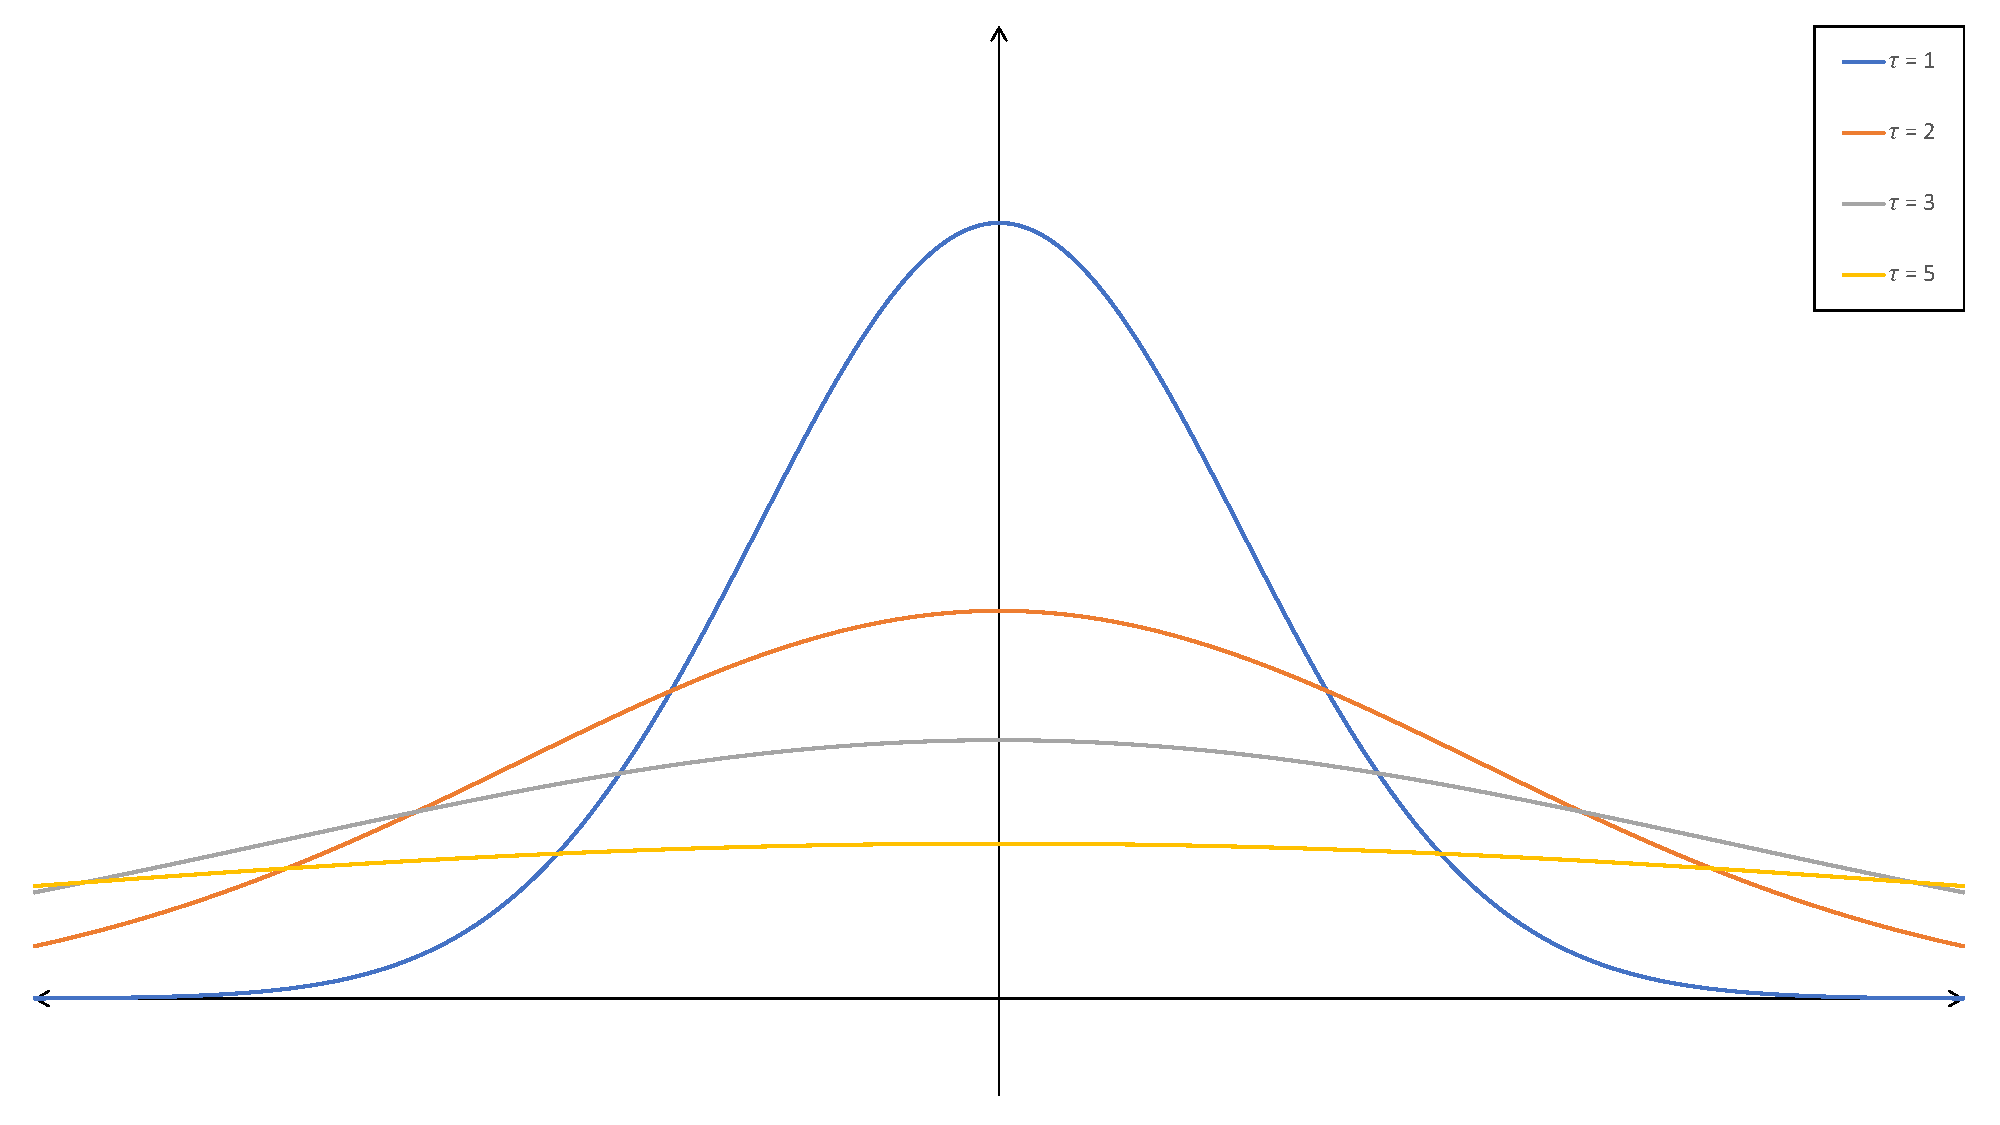
\includegraphics[width=\linewidth]{figure/Lecture08/fig-2.pdf}
\end{figure}

First, as $n \rightarrow \infty$, the first term in \eqref{8.64} dominates the second term. As we would hope, as the size of our dataset grows the influence of the prior on the posterior of $\theta$ diminishes and, at the limit, vanishes. For this reason, Bayesian methods are less useful under a large data regime. Second, as $\tau \rightarrow \infty$, our Gaussian prior becomes increasingly flat and uninformative; see Figure 8.2. Accordingly, in \eqref{8.64}, $\tau$ is inversely related to the influence of the prior on the posterior. Third, the variance of our posterior predictive distribution $y^* \mid x^*, S$ is at least $\sigma^2$. 

\begin{proof}
First, we show that $A$ is positive definite. For non-zero $z \in \R^d$, 
\als{
z^\top \frac{1}{\sigma^2}X^\top X z &= \frac{1}{\sigma^2} (Xz)^\top Xz\\
&= \frac{1}{\sigma^2} \langle Xz, Xz, \rangle. \label{8.66}
}
Since $X$ is full-rank (our predictors cannot be a linear combination of each other), $X$'s null space is trivial and $Xz \neq 0$. Because $\sigma^2$ is positive and the norm is positive for all non-zero vectors, \eqref{8.66} is positive and $A$ is positive definite. Then, $A^{-1}$ is also positive definite since its eigenvalues are the reciprocals of $A$'s eigenvalues.\footnote{For any invertible matrix $M$, $M^{-1}$'s eigenvalues are the eigenvalues of $M$ inverted. A matrix is positive definite if and only if all of its eigenvalues are positive \cite{axler_linear_2014}.} Thus, 
\als{
{x^*}^\top A^{-1}x^{*} + \sigma^2 \geq \sigma^2.
}
\end{proof}
As expected, our uncertainty regarding our predictions is bounded below by $\sigma^2$, which is the uncertainty intrinsic to the problem. Moreover, as our dataset grows in observations, we approach this lower bound and achieve it at the infinite limit. As $n \rightarrow \infty$, ${x^*}^\top A^{-1}x^* \rightarrow 0$, since as $n \rightarrow \infty$, $A \rightarrow \infty$.  